% Select IEEEtran's Times font encoding before the class loads (also for XeTeX).
\RequirePackage[T1]{fontenc}
\documentclass[conference]{IEEEtran}
% \IEEEoverridecommandlockouts
% The preceding line is only needed to identify funding in the first footnote. If that is unneeded, please comment it out.
\usepackage{cite}
\usepackage{amsmath,amssymb,amsfonts}
\usepackage{graphicx}
\usepackage[caption=false,font=footnotesize]{subfig}
\usepackage{comment}
\usepackage{textcomp}
\usepackage{tabularx}
\usepackage{booktabs}
\usepackage{listings}
\usepackage{xcolor}
\usepackage{url}

\def\BibTeX{{\rm B\kern-.05em{\sc i\kern-.025em b}\kern-.08em
    T\kern-.1667em\lower.7ex\hbox{E}\kern-.125emX}}
\begin{document}

\title{Learning Direction-Specific Cross-Modal Interactions for Visual Question Answering}

\author{\IEEEauthorblockN{Aditya Katre}
\IEEEauthorblockA{\textit{High School Student, Del Norte High School} \\
San Diego, United States of America \\
adityapkatre@gmail.com}
\and
\IEEEauthorblockN{Hajar Homayouni}
\IEEEauthorblockA{\textit{Department of Computer Science} \\
\textit{San Diego State University}\\
San Diego, United States of America \\
hhomayouni@sdsu.edu}
% \and
% \IEEEauthorblockN{3\textsuperscript{rd} Given Name Surname}
% \IEEEauthorblockA{\textit{dept. name of organization (of Aff.)} \\
% \textit{name of organization (of Aff.)}\\
% City, Country \\
% email address or ORCID}
}

\maketitle

\begin{abstract}
Multimodal representation learning requires models to fuse heterogeneous information sources, such as images and text. However, many existing fusion methods use symmetric cross-modal interaction mechanisms that treat image-to-text and text-to-image interactions as equivalent, even though these directions can serve different functional roles. In this paper, we propose an asymmetric cross-modal learning framework that uses independent cross-attention modules for each direction of multimodal exchange, enabling direction-specific representations for multimodal reasoning. We evaluate the framework on VQA v2.0 against a parameter-matched symmetric baseline, including frozen-encoder experiments, multi-seed evaluation, modality-blind ablations, and question-type analysis. Modality-blind ablations show accuracy drops when either modality input is removed. Results show a modest advantage for the tested asymmetric architecture compared to a parameter-matched symmetric baseline, and that gains were positive in all six comparisons on the full validation set. These findings suggest that direction-specific cross-modal attention has a small, consistent advantage under equal parameter counts.
\end{abstract}

\begin{IEEEkeywords}
Multimodal learning, Cross-modal attention, Asymmetric fusion, Vision-language reasoning, Visual question answering.
\end{IEEEkeywords}

\section{Introduction}
Multimodal learning aims to integrate heterogeneous sources of information, or modalities, such as images, text, audio, and structured signals, into a unified representation that supports reasoning across complementary views of the same problem~\cite{baltrusaitis2019multimodal,ramachandram2017deep}. In visual question answering (VQA), an image provides visual evidence while a natural-language question specifies what information should be extracted from that image~\cite{antol2015vqa,goyal2017making}. A central challenge in multimodal representation learning is therefore how modalities should interact.

Existing multimodal fusion strategies are commonly grouped into early, late, and mid-level fusion~\cite{baltrusaitis2019multimodal,ramachandram2017deep}. Early fusion combines modalities at the raw-input or low-level feature stage. This simple strategy can capture fine-grained correlations between modalities, but it can also create high-dimensional representations, increase computational cost, and make the model sensitive to modality imbalance, where one modality dominates learning. Late fusion, in contrast, trains separate unimodal models and combines their predictions through mechanisms such as averaging, voting, or learned decision-level aggregation. This modular approach reduces negative interference between modalities, but provides limited opportunity for cross-modal reasoning because interactions occur after each modality produces independent outputs. Mid-level fusion offers a balance between these two extremes by first encoding each modality independently and then learning interactions between their intermediate representations. This design enables reasoning across modalities, making it suitable for tasks that require alignment between language and visual evidence.

Many mid-fusion architectures still use symmetric interaction mechanisms, where the same transformation or shared module is applied to both directions of modality exchange. This implicitly assumes that modality $A$ attending to modality $B$ requires the same representational behavior as modality $B$ attending to modality $A$. However, modalities often have different structures and roles: text is discrete and task-specifying, while images are spatial and evidence-bearing. Thus, a question attending to an image may need to localize relevant visual regions, whereas an image attending to a question may need to identify the linguistic constraints that guide interpretation. Sharing parameters across these directions can therefore limit the model's ability to learn direction-specific relationships.

In this paper, we evaluate independent directional cross-attention modules on VQA v2.0 using pretrained image and text encoders. We compare the proposed architecture with a symmetric control with the same parameter count.
The main contributions of this work are as follows:
\begin{itemize}
\item We introduce an asymmetric cross-modality learning framework that models directional multimodal interactions using independent cross-attention modules rather than shared symmetric interaction weights.
\item We evaluate both architectures across three paired seeds for frozen and fully fine-tuned encoders, and report test results. 
\item We examine dependence on each modality and differences across official VQA v2.0 answer types to examine the scope of gains.
\end{itemize}

Implementation code is available at: \url{https://github.com/adikatre/Asymmetric-Cross-Modal-Attention.git}

\section{Related Work}
A major direction in multimodal learning is aligning different modalities in a shared embedding space. CLIP learns transferable visual representations through image-text contrastive pretraining~\cite{radford2021learning}. Cross-modal attention is widely used for aligning modalities. For example, LAVISH routes cross-modal exchange through compact latent tokens to reduce full cross-attention cost~\cite{lin2023lavish} and MutualFormer estimates cross-modal affinities through intra-modality structure to address modality gaps~\cite{hu2024mutualformer}. These approaches demonstrate the value of explicit interaction, but they do not directly test whether opposite directions, such as image-to-text and text-to-image, should share the same attention parameters.

Asymmetric fusion has been explored in RGB-D semantic segmentation, remote sensing, image-text retrieval, video moment retrieval, medical VQA, and explainable VQA~\cite{du2024asymformer,aafremotesensing,ascl,asymmetricvideomoment,acma,li2025mrvqa}. These methods show that modalities can contribute unequal or direction-dependent information. However, most introduce asymmetry through task-specific designs. Thus, although effective, these approaches often couple asymmetry with domain-specific architectures, auxiliary objectives, augmentation strategies, or explanation modules.


\section{Proposed Approach}

We propose an asymmetric multimodal learning framework for modeling directional relationships between images and questions. Let $\mathbf{X}^{A}$ and $\mathbf{X}^{B}$ denote the image and text inputs. Each modality is encoded independently and projected into a shared latent dimension:
\[
\mathbf{Z}^{A}=\phi_A(E_A(\mathbf{X}^{A})), \qquad
\mathbf{Z}^{B}=\phi_B(E_B(\mathbf{X}^{B}))
\]
where $E_A$ and $E_B$ are modality-specific encoders and $\phi_A$ and $\phi_B$ are learnable projections.
\[
\mathrm{Attn}(\mathbf{Q},\mathbf{K},\mathbf{V})
=\mathrm{softmax}\left(\frac{\mathbf{Q}\mathbf{K}^{T}}{\sqrt{d_k}}\right)\mathbf{V},
\]
where $d_k$ is the key dimension. In cross-attention, the querying modality supplies $\mathbf{Q}$, while the other modality supplies $\mathbf{K}$ and $\mathbf{V}$. Each block includes learned attention projections, layer normalization, residual connections, and a feed-forward network.

The asymmetric fusion module uses separate blocks to independently query each modality:

\[
\begin{aligned}
\widehat{\mathbf{Z}}^{A}
&=
F_A\left(
\mathbf{Q}=\mathbf{Z}^{A},
\mathbf{K}=\mathbf{Z}^{B},
\mathbf{V}=\mathbf{Z}^{B}
\right),\\
\widehat{\mathbf{Z}}^{B}
&=
F_B\left(
\mathbf{Q}=\mathbf{Z}^{B},
\mathbf{K}=\mathbf{Z}^{A},
\mathbf{V}=\mathbf{Z}^{A}
\right).
\end{aligned}
\]
\noindent The parameter sets of $F_A$ and $F_B$ are independent. The first cross-attention module produces the updated representation $\widehat{\mathbf{Z}}^A$, which is the representation of modality $A$ attending to modality $B$. The second module produces $\widehat{\mathbf{Z}}^B$, the representation of modality $B$ attending to modality $A$.

Therefore, $\mathbf{Z}^{B}$ is used as the query, while $\mathbf{Z}^{A}$ is used as both the key and the value:
\[
\mathbf{Q}_{B \rightarrow A} = \mathbf{Z}^{B}, \qquad
\mathbf{K}_{B \rightarrow A} = \mathbf{Z}^{A}, \qquad
\mathbf{V}_{B \rightarrow A} = \mathbf{Z}^{A}.
\]
\[
\begin{aligned}
\left(
\widehat{\mathbf{Z}}^{B},
\mathbf{M}_{B \rightarrow A}
\right)
&=
\mathrm{CrossAttn}_{B \rightarrow A}
\left(
\mathbf{Q}_{B \rightarrow A},
\right. \\
&\hspace{0.18in}
\left.
\mathbf{K}_{B \rightarrow A},
\mathbf{V}_{B \rightarrow A}
\right).
\end{aligned}
\]

\noindent The second cross-attention module produces the updated representation $\widehat{\mathbf{Z}}^{B}$ and the attention map $\mathbf{M}_{B \rightarrow A}$. Here, $\widehat{\mathbf{Z}}^{B}$ is the representation of modality $B$ after incorporating information from modality $A$. The attention map $\mathbf{M}_{B \rightarrow A}$ shows how strongly each token or feature in modality $B$ attends to each token or feature in modality $A$.

Unlike a symmetric fusion design (see symmetric vs. asymmetric designs in Figure~\ref{sym-vs-asym}), the two cross-attention modules $\mathrm{CrossAttn}_{A \rightarrow B}$ and $\mathrm{CrossAttn}_{B \rightarrow A}$ do not share parameters. This allows each direction to learn its own query, key, value, and output transformations. As a result, the framework can specialize the two directions for different functional roles.
The attended representations are then aggregated and combined:
\[
\mathbf{r}^{A} = \mathrm{Pool}(\widehat{\mathbf{Z}}^{A}), \qquad
\mathbf{r}^{B} = \mathrm{Pool}(\widehat{\mathbf{Z}}^{B}).
\]

\noindent The final fused representation is obtained by concatenating the two direction-specific representations:
\begin{equation}
\mathbf{r}^{AB} = [\mathbf{r}^{A}; \mathbf{r}^{B}],
\end{equation}
where $[\cdot;\cdot]$ denotes concatenation. The fused representation $\mathbf{r}^{AB}$ is then passed to a task-specific prediction head:
\[
\widehat{y} = g(\mathbf{r}^{AB}).
\]

\noindent The task head can be adapted to classification, answer prediction, retrieval scoring, or other downstream multimodal objectives.



To isolate the contribution of asymmetric fusion, we compare the proposed framework with a symmetric baseline. The parameter-matched symmetric baseline uses the same encoders, projection layers, pooling strategy, prediction head, optimizer, and training setup as the asymmetric model. Both models have two cross-attention blocks and the same number of fusion parameters (6,306,816). The asymmetric model uses two independent directional blocks, with one block assigned to each direction. The symmetric baseline uses two shared cross-attention blocks: each block is applied to both image-to-text and text-to-image directions, and both outputs are averaged. The symmetric baseline uses four cross-attention calls, while the asymmetric model uses two. Therefore, the comparison focuses on the asymmetric vs. symmetric fusion, but is parameter-matched, not compute-matched.

\begin{figure}[!t]
\centering
\subfloat[Symmetric cross-modal fusion baseline.\label{fig:symmetric}]{%
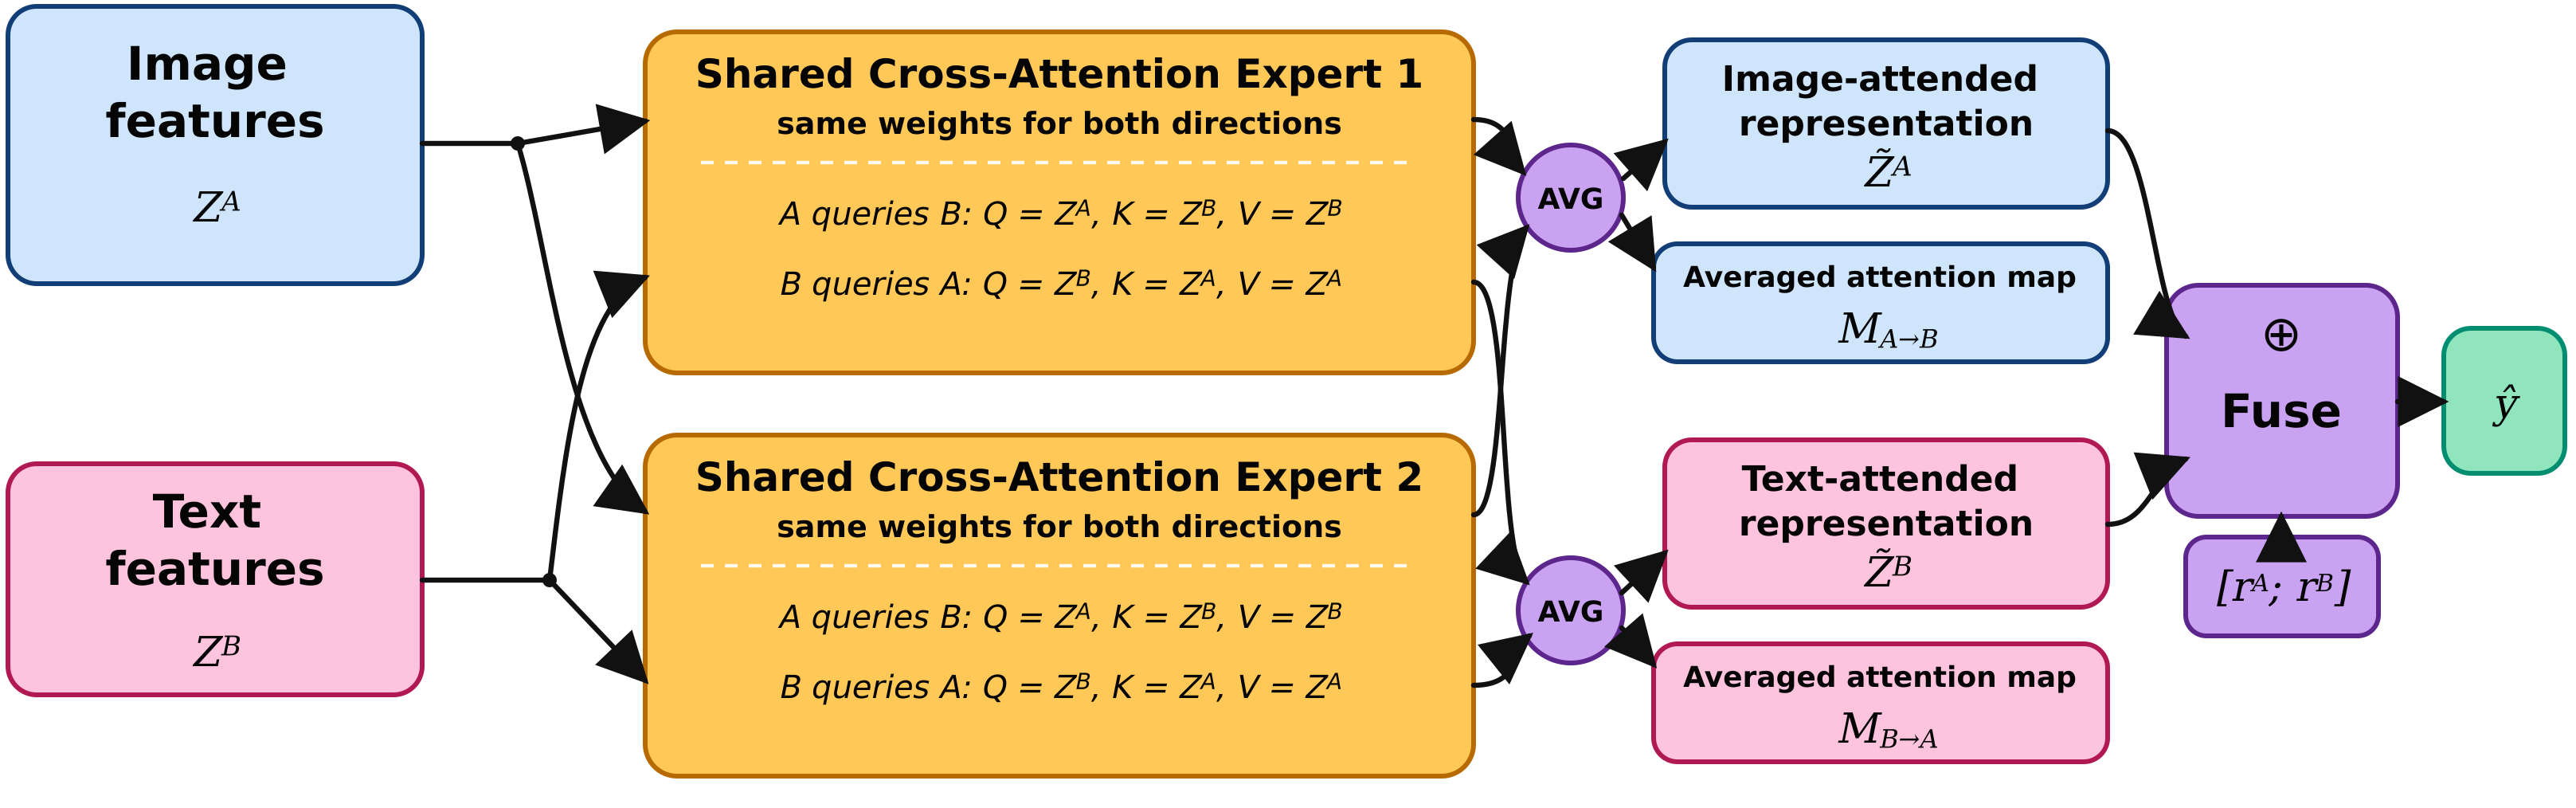
\includegraphics[width=\linewidth]{symmetric.png}}
\par
\subfloat[Asymmetric cross-modal fusion framework.\label{fig:asymmetric}]{%
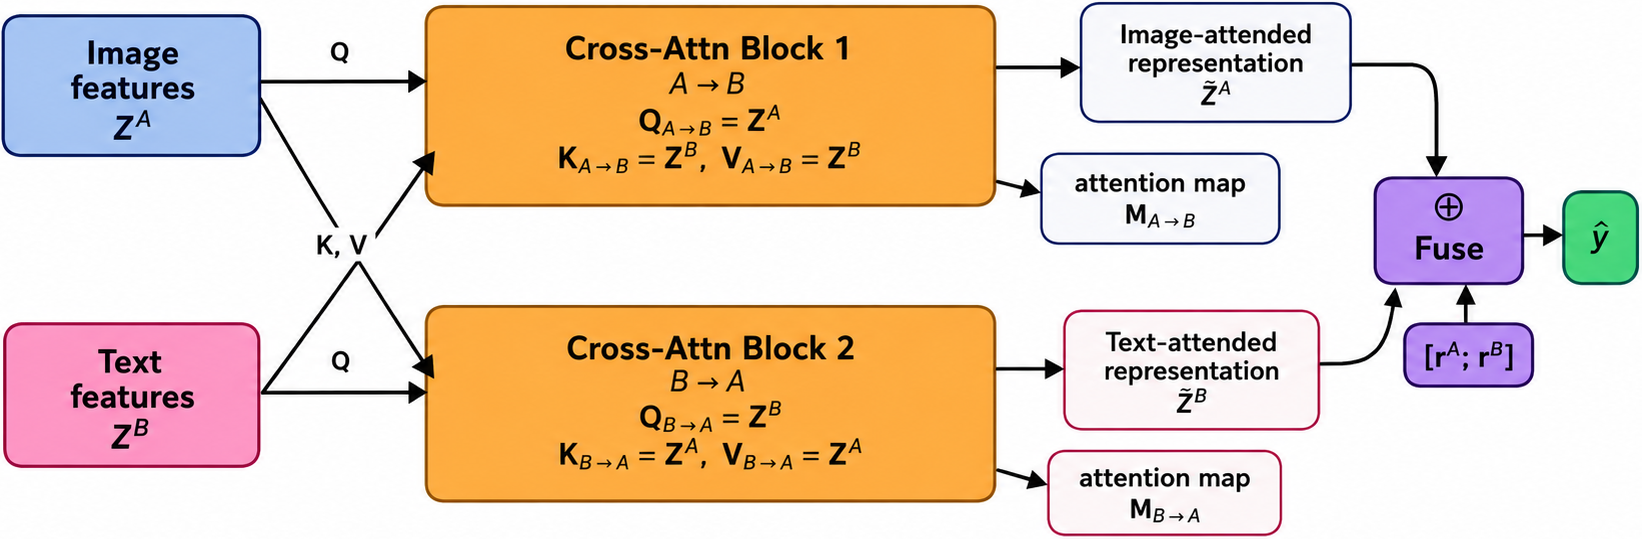
\includegraphics[width=\linewidth]{asymmetric.png}}
\caption{Symmetric vs. Asymmetric Cross-modal Fusion.}
\label{sym-vs-asym}
\end{figure}

\section{Implementation of the Framework}

The implementation uses Vision Transformer with a patch size of 32 (CLIP ViT-B/32) for images along with RoBERTa-base for text. The CLIP ViT-B/32 encoder divides each input image into non-overlapping $32 \times 32$ patches. For a $224 \times 224$ image, this produces 49 image patch embeddings. A \texttt{[CLS]} token is then appended to the patch sequence, resulting in 50 visual tokens. The text input is encoded using RoBERTa-base, which produces contextualized token-level representations for the input sentence or question.

Before fusion, the visual and textual encoder outputs are projected into a shared 512-dimensional latent space using learnable linear projection layers. This projection step ensures that both modalities have the same embedding dimension before they are passed to the cross-modal attention modules. The resulting projected visual and textual representations correspond to $\mathbf{Z}^{A}$ and $\mathbf{Z}^{B}$ in the proposed framework.

Each CrossAttention block follows a pre-normalization Transformer-style design. Given a query sequence from one modality and key/value sequences from the other modality, the block applies multi-head cross-attention followed by a feed-forward neural network. Residual connections and dropout are used to stabilize optimization and reduce overfitting. In our implementation, each cross-attention block uses 8 attention heads. The attended representations from the two directions are then pooled, concatenated, and passed to a task-specific prediction layer. 

\noindent The concatenated fused representation is passed through an MLP classifier with dropout, followed by a final linear projection to the answer space. 

\subsection{Hyperparameter Configuration}

\begin{table}[t]
\centering
\caption{Hyperparameter and training configuration for VQA v2.0. Unfrozen denotes fully fine-tuning both encoders.}
\label{tab:hparams}
\small
\setlength{\tabcolsep}{4pt}
\renewcommand{\arraystretch}{1.12}
\begin{tabular}{p{0.48\columnwidth}cc}
\hline
\textbf{Hyperparameter} & \textbf{Frozen} & \textbf{Unfrozen} \\
\hline
Embedding dimension & 512 & 512 \\
Attention heads & 8 & 8 \\
Dropout rate & 0.1 & 0.1 \\
Batch size & 2,048 & 128 \\
Projection/fusion/head LR & $2\times10^{-4}$ & $2\times10^{-4}$ \\
Encoder learning rate & N/A& $2\times10^{-6}$ \\
Weight decay & $10^{-2}$ & $10^{-2}$ \\
Warmup epochs & 0 & 1 \\
Training epochs & 12 & 12 \\
Answer vocabulary size & 3,000 & 3,000 \\
Maximum question length & 20 tokens & 20 tokens \\
\hline
\end{tabular}
\end{table}

Table~\ref{tab:hparams} summarizes the hyperparameter configuration used for the experiments. The same configuration is used for both the symmetric and asymmetric fusion models to ensure a controlled comparison. These hyperparameters were selected for a single NVIDIA A100 GPU with 40 GB of memory. For the frozen-encoder experiments, the encoder outputs do not change across epochs, so visual and textual features are extracted offline and reused during training. The answer vocabulary is reduced to contain the 3,000 most frequent training answers. For every seed, the best epoch was selected using the official VQA v2.0 accuracy on all 214,354 validation questions. For test submission for the hidden test set on the EvalAI leaderboard, the highest-scoring checkpoint was chosen for each architecture (Asymmetric/Symmetric) and encoder setting (Frozen/Unfrozen).


\subsection{Dataset \& Evaluation Method}

\noindent VQA v2.0~\cite{goyal2017making} is a visual question answering benchmark in which each example consists of an image, a natural-language question, and multiple human-provided answers.  It contains natural images from MS-COCO (Microsoft Common Objects in Context) paired with questions and human-generated answers. The task requires the model to answer questions regarding images. The two modalities in the data play distinct roles: the question specifies what should be extracted, while the image provides the evidence. In our implementation, the answer space is restricted to the 3,000 most frequent answers. The training, validation, and test splits contain 443,757, 214,354, and 447,793 questions for 82,783, 40,504, and 81,434 images, respectively. Every annotation also includes an \textit{answer\_type} label to denote the type of question, such as yes/no, number, or other.

Evaluation uses the VQA v2.0 consensus score to account for variation among 10 human-generated annotations for each image-question pair~\cite{antol2015vqa}.  For a normalized prediction $\hat{a}$ and ten normalized human answers $a_1,\ldots,a_{10}$, the score is
\begin{equation}
s(\hat{a})=\frac{1}{10}\sum_{i=1}^{10}
\min\left(1,\frac{\sum_{j\neq i}\mathbf{1}[\hat{a}=a_j]}{3}\right).
\end{equation}
The overall accuracy is the average question score expressed as a percentage.

\section{Evaluation}

We evaluate whether the proposed asymmetric cross-modal fusion framework improves VQA accuracy compared to the parameter-matched symmetric model, whether the observed difference persists across seeds and encoder settings, and the effect on performance when an input modality is removed.

\subsection{VQA Performance Across Seeds and Encoder Settings}

Table~\ref{tab:vqa_answer_prediction} reports validation accuracy as a mean $\pm$ standard deviation for three seeds (7, 42, and 123). The asymmetric model achieves $59.77 \pm 0.20\%$ with frozen encoders, compared with $59.29 \pm 0.18\%$ for the Symmetric Parameter-matched (PM) baseline. With unfrozen encoders, the corresponding accuracies are $65.53 \pm 0.07\%$ and $65.30 \pm 0.09\%$. These are small mean improvements: $0.48 \pm 0.19$ percentage points with frozen encoders and $0.23 \pm 0.16$ points with fully fine-tuned, or unfrozen, encoders.

\begin{table}[t]
\centering
\caption{VQA validation accuracy (\%) on all 214,354 questions. Results are mean $\pm$ standard deviation across three paired seeds. Gain is the paired asymmetric-minus-symmetric difference in percentage points.}
\label{tab:vqa_answer_prediction}
\setlength{\tabcolsep}{3pt}
\renewcommand{\arraystretch}{1.05}
\begin{tabular}{lccc}
\hline
\textbf{Encoders} & \textbf{Symmetric} & \textbf{Asymmetric} & \textbf{Gain (pp)}\\
\hline
Frozen & $59.29\pm0.18$ & $59.77\pm0.20$ & $+0.48\pm0.19$\\
Unfrozen & $65.30\pm0.09$ & $65.53\pm0.07$ & $+0.23\pm0.16$\\
\hline
\end{tabular}
\end{table}

\subsection{Hidden Test Dataset Results}

Table~\ref{tab:vqa_test} reports final EvalAI results for the selected checkpoints. Asymmetric fusion improves test-standard accuracy from $61.29\%$ to $61.61\%$ with frozen encoders and from $67.13\%$ to $67.54\%$ with unfrozen encoders.  We chose checkpoints with the highest validation-subset scores and used them to perform inference for the hidden test dataset.

\begin{table}[t]
\centering
\caption{EvalAI VQA accuracy (\%) for individual checkpoints selected with highest validation-subset scores.}
\label{tab:vqa_test}
\setlength{\tabcolsep}{3pt}
\renewcommand{\arraystretch}{1.05}
\begin{tabular}{llccc}
\hline
\textbf{Encoders} & \textbf{Model} & \textbf{Seed} & \textbf{Test-dev} & \textbf{Test-std}\\
\hline
Frozen & Symmetric& 7 & 60.97 & 61.29\\
Frozen & Asymmetric& 42 & 61.35& 61.61\\
Unfrozen & Symmetric& 42 & 66.78 & 67.13\\
Unfrozen & Asymmetric& 42 & 67.00& 67.54\\
\hline
\end{tabular}
\end{table}

\subsection{Dependence on Both Modalities}

We test whether the models use both modalities or rely on unimodal shortcuts. We conduct modality-blind ablations by zeroing out one modality at a time and evaluating. In the image-blind condition, image features are replaced with zeros, forcing the model to rely on the question and answer distribution. In the text-blind condition, text features are replaced with an attention mask, forcing the model to predict without the question. Text-blind has a larger drop for all four settings below, so both models depend more on the question than on the image.


\begin{table}[t]
\centering
\small
\caption{Modality-blind VQA accuracy (\%) on the fixed 10,000-question validation subset. Frozen seeds are 7 for Symmetric (parameter matched) and 42 for Asymmetric; both unfrozen models use seed 42.}
\label{tab:vqa_modality_ablation}
\setlength{\tabcolsep}{3pt}
\renewcommand{\arraystretch}{1.05}
\begin{tabular}{llcc}
\hline
\textbf{Encoders} & \textbf{Condition} & \textbf{Sym.-PM} & \textbf{Asym.}\\
\hline
Frozen & Full input & 60.62 & 61.18\\
Frozen & Image-blind & 25.50 & 24.34\\
Frozen & Text-blind & 12.69 & 19.83\\
\hline
Unfrozen & Full input & 65.92 & 66.35\\
Unfrozen & Image-blind & 32.81 & 33.17\\
Unfrozen & Text-blind & 25.30 & 25.09\\
\hline
\end{tabular}
\end{table}

Table~\ref{tab:vqa_modality_ablation} shows major drops across all image-blind and text-blind conditions for the Symmetric Parameter Matched Baseline and the Asymmetric models. These results indicate that both models depend on images and questions jointly.

\subsection{Answer-Type Analysis}

We examine the official yes/no, number, and other answer types on test-standard split for the highest selected checkpoints on each model variant.

\begin{table}[t]
\centering
\caption{Test-standard VQA accuracy (\%) by answer type
for selected checkpoints. $\Delta$ is asymmetric minus symmetric,
in percentage points.}
\label{tab:vqa_answer_types}
\setlength{\tabcolsep}{3pt}
\renewcommand{\arraystretch}{1.05}
\begin{tabular}{llrrr}
\hline
\textbf{Encoders} & \textbf{Type} & \textbf{Symmetric}& \textbf{Asymmetric}& $\boldsymbol{\Delta}$ \\
\hline
Frozen & Yes/no & 77.09 & \textbf{77.41} & +0.32 \\
Frozen & Number & 40.57 & \textbf{41.02} & +0.45 \\
Frozen & Other  & 52.29 & \textbf{52.57} & +0.28 \\
\hline
Unfrozen & Yes/no & 83.49 & \textbf{83.90} & +0.41 \\
Unfrozen & Number & \textbf{45.60} & 45.34 & $-0.26$ \\
Unfrozen & Other  & 57.83 & \textbf{58.37} & +0.54 \\
\hline
\end{tabular}
\end{table}

Table~\ref{tab:vqa_answer_types} shows that the asymmetric model achieves higher test-standard accuracy across all three answer types with frozen encoders. The largest observed gain is for number answers, at 0.45 percentage points. With unfrozen encoders, asymmetric fusion improves yes/no and other accuracy by 0.41 and 0.54 points, respectively, while number accuracy decreases by 0.26 points. Thus, the overall asymmetric advantage includes gains in several answer types, but the pattern varies across encoder settings. These results describe selected checkpoints and do not establish statistically significant differences within individual answer types.

\subsection{Comparison with Large-Scale Multimodal Baselines}

Recent large-scale multimodal systems have achieved strong performance by combining massive pretraining datasets, large vision and language backbones, and substantial computational resources. For example, CLIP learns transferable image-text representations from 400 million image-text pairs~\cite{radford2021learning}; Flamingo enables few-shot vision-language learning over interleaved image, video, and text inputs~\cite{alayrac2022flamingo}; BLIP-2 connects frozen image encoders with frozen large language models through a lightweight Querying Transformer~\cite{li2023blip2}; and LLaVA demonstrates the effectiveness of visual instruction tuning for general-purpose multimodal understanding~\cite{liu2023visual}. These models provide important reference points for multimodal learning, but directly competing with them is difficult under the limited computational and data resources available in this study. Our goal is therefore not to outperform large-scale foundation models, but to isolate a specific architectural question: whether opposite directions of cross-modal interaction should share parameters. By controlling the encoders, training setup, and symmetric baseline, our experiments show when direction-specific fusion is useful. 

\section{Limitations and Mitigation Strategies}

Matching the learned fusion parameter budget does not necessarily imply identical computational cost or optimization dynamics. Symmetric-PM controls learned capacity while retaining shared directional transformations, but the symmetric and asymmetric architectures may still differ in how those parameters are applied during the forward pass. A stricter future control could additionally match floating-point operations, effective depth, memory use, and inference latency.


The comparison is parameter-matched but not compute-matched. Both architectures contain 6{,}306{,}816 learned fusion parameters, so the observed accuracy differences cannot be attributed to greater fusion capacity in the asymmetric model. However, the asymmetric model applies one independent block in each direction, requiring two cross-attention calls, whereas the symmetric control applies both shared experts in both directions, requiring four calls. As a result, the symmetric control requires more computation than the asymmetric model. Therefore, the models have an equal number of parameters, but differ in computational cost.


Additionally, parameter matching establishes that the residual performance advantage cannot be explained by learned fusion capacity alone, but it does not directly identify what the two directional attention modules learn differently. Future work could examine attention distributions, representation similarity, direction-specific projection weights, or module ablations to characterize the functional specialization learned by the two directions.

\section{Conclusion}

This work studied whether cross-modal fusion should treat opposite directions of multimodal interaction as equivalent. We introduced an asymmetric fusion framework that uses independent cross-attention modules for image-to-text and text-to-image exchange, allowing each direction to learn its own role in multimodal reasoning.


The results suggest that direction-specific cross-modal fusion provides modest benefits for visual question answering with both frozen and fine-tuned (unfrozen) encoders. These benefits vary across answer types. Modality-blind ablations indicate that both architectures rely on visual and textual information. Overall, the findings support further exploration of independent directional approaches for multimodal learning.

\bibliographystyle{IEEEtran}
\bibliography{references}

\end{document}